\chapter{Study of R-hadron treatment in simulation}
\label{r_hadrons}

In the $\Pp\Pp {\to} \PSQt \PASQt$ signal processes, the top squarks can form strongly produced \linebreak[4]hadronic states called ``R-hadrons.'' In the $\PSQt {\to} \cPqb \Pl$ and $\PSQt {\to} \cPqd \Pl$ signal samples used in this analysis, R-hadron formation and decay are modeled with \PYTHIA while the R-hadron interactions with material are not modeled. Given that the the lepton identification criteria effectively limit the number of interaction lengths an R-hadron can traverse before decaying, we expect the impact of such interactions to be negligible. To test this hypothesis, we generate alternative signal samples in which the R-hadron material interactions and decay are modeled in \GEANTfour and compare the resulting signal efficiency to that of the nominal samples. We find differences in signal efficiency on the order of 20\% that are completely attributable to differences in the treatment of jet formation between the \PYTHIA and \GEANTfour implementations and therefore conclude that the R-hadron material interactions do not meaningfully impact the analysis.

In the alternative samples, the R-hadron interactions are modeled following the ``cloud model'', which assumes that the top squark is surrounded by a cloud of colored, light constituents that interact during scattering~\cite{mackeprang_2006,mackeprang_2009}. Such interactions can potentially alter the rate of R-hadron energy loss or cause the R-hadron charge value to change mid-flight. In the context of CMSSW, simultaneously enabling R-hadron interactions with material and R-hadron decay within the detector volume constrains us to perform both the R-hadron propagation and decay with \GEANTfour. We generate two additional sets of signal samples for this study. In the first, the R-hadron decays to a lepton and bottom quark. Because \GEANTfour does not perform the parton shower and hadronization that lead to jet formation, the bottom quark is in this case unrealistically treated as a final-state particle. To help study the effect of this missing jet formation, we generate a second sample in which the R-hadron decays to a lepton and a neutral pion, which then decays to two photons and initiates an electromagnetic shower.

Figure~\ref{r_hadron_cutflows} shows how modeling the R-hadron interactions and decay in \GEANTfour affects the inclusive signal region cutflows in the $\Pe\Pe$ and $\Pgm\Pgm$ channels. The alternative samples generally pass the full selection at a slightly higher rate than the existing signal samples. The overall magnitude of the effect is similar across channels and signal points, and a few clear trends are apparent in the cutflows. First, events from the neutral pion sample pass the $\Pe\Pe$ trigger at a higher rate than other samples because of the increased number of high-momentum photons and electrons from the neutral pion decay, an effect that carries through the full selection. Second, $\PSQt {\to} \cPqb \Pl$ events pass the $\Pgm\Pgm$ trigger at a higher rate due to the increased number of muons from b jets, but this effect is neutralized by the muon isolation criteria. Third, events in which the R-hadron decays to a lepton and a final-state b quark in \GEANTfour pass the $\Pe\Pe$ trigger at lower rates due to the reduced number of electrons from jets but pass the lepton quality and isolation criteria at higher rates because the absence of jets increases the probability that leptons from the top squark decay are well isolated. A similar effect can be seen in the neutral pion sample in the $\Pgm\Pgm$ cutflow. The effects on electrons and muons identified in the same-flavor channels are also apparent in the $\Pe\Pgm$ channel.

\begin{figure}
\centering
%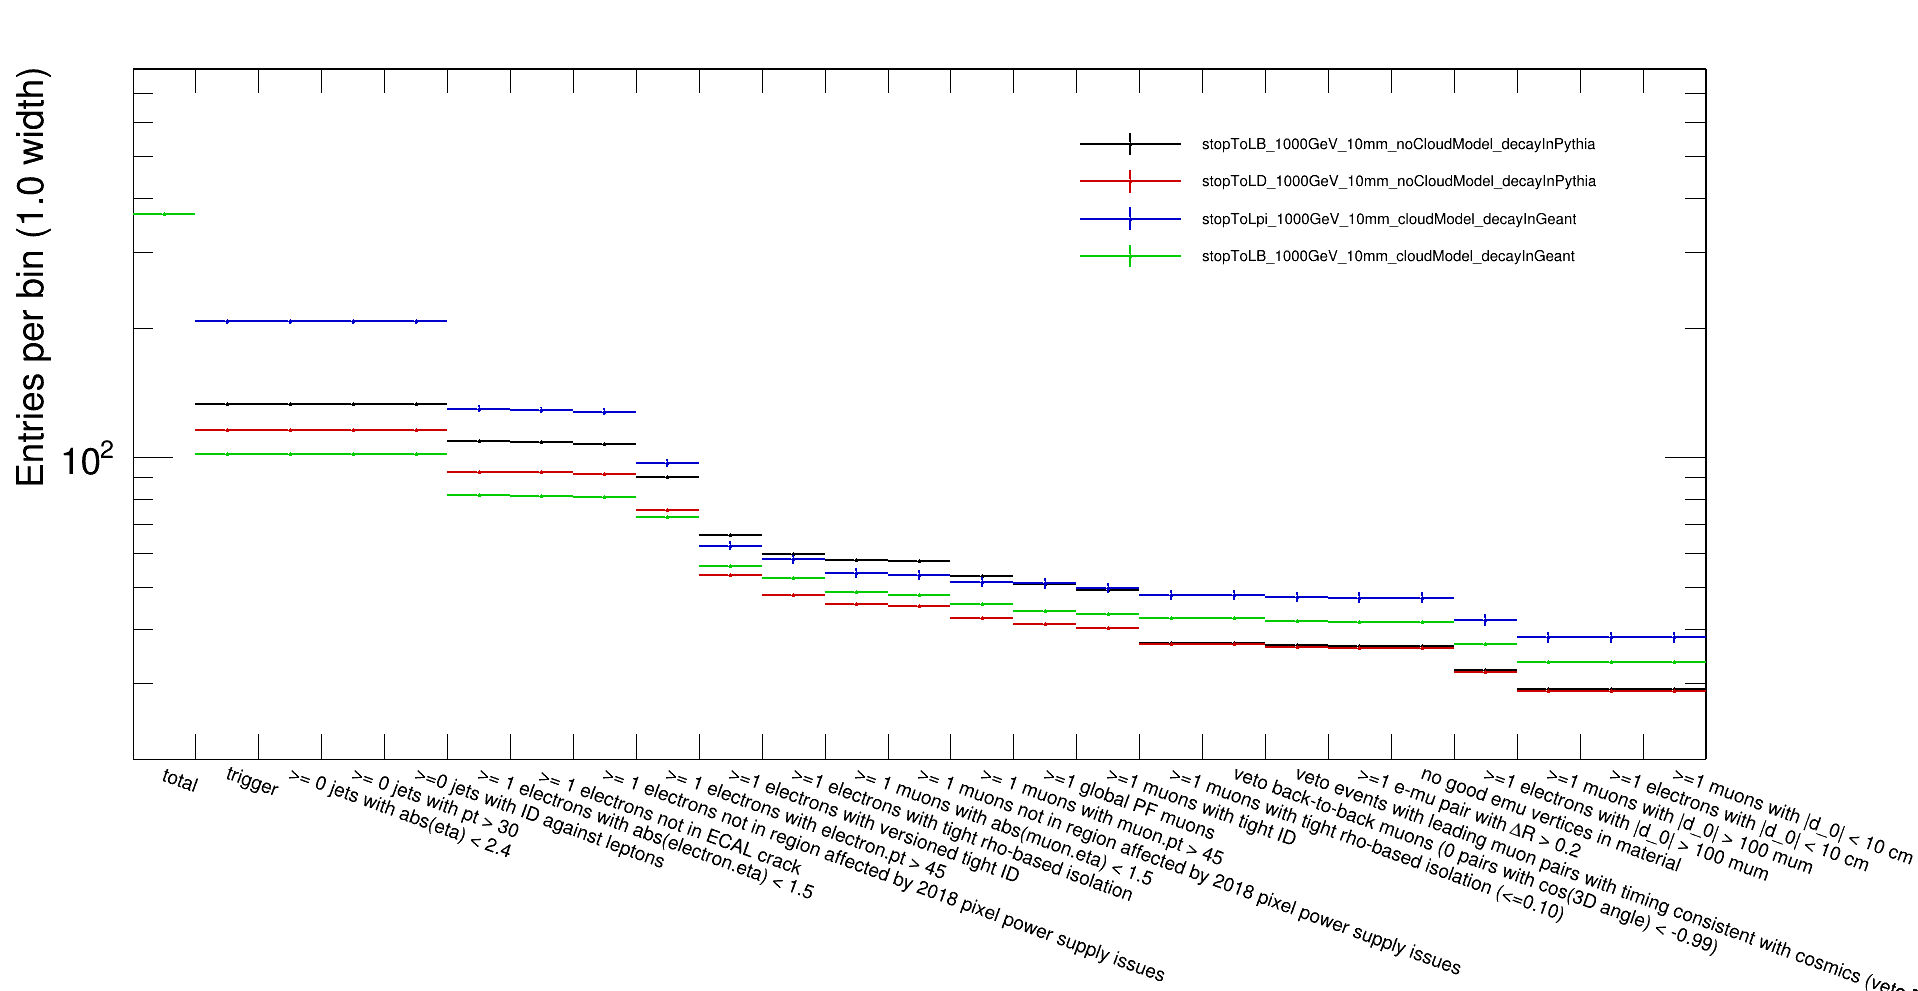
\includegraphics[width=0.78\textwidth]{figures/r_hadrons/emu_cutFlows_lb_ld_lpi_l_1000GeV_10mm.pdf}
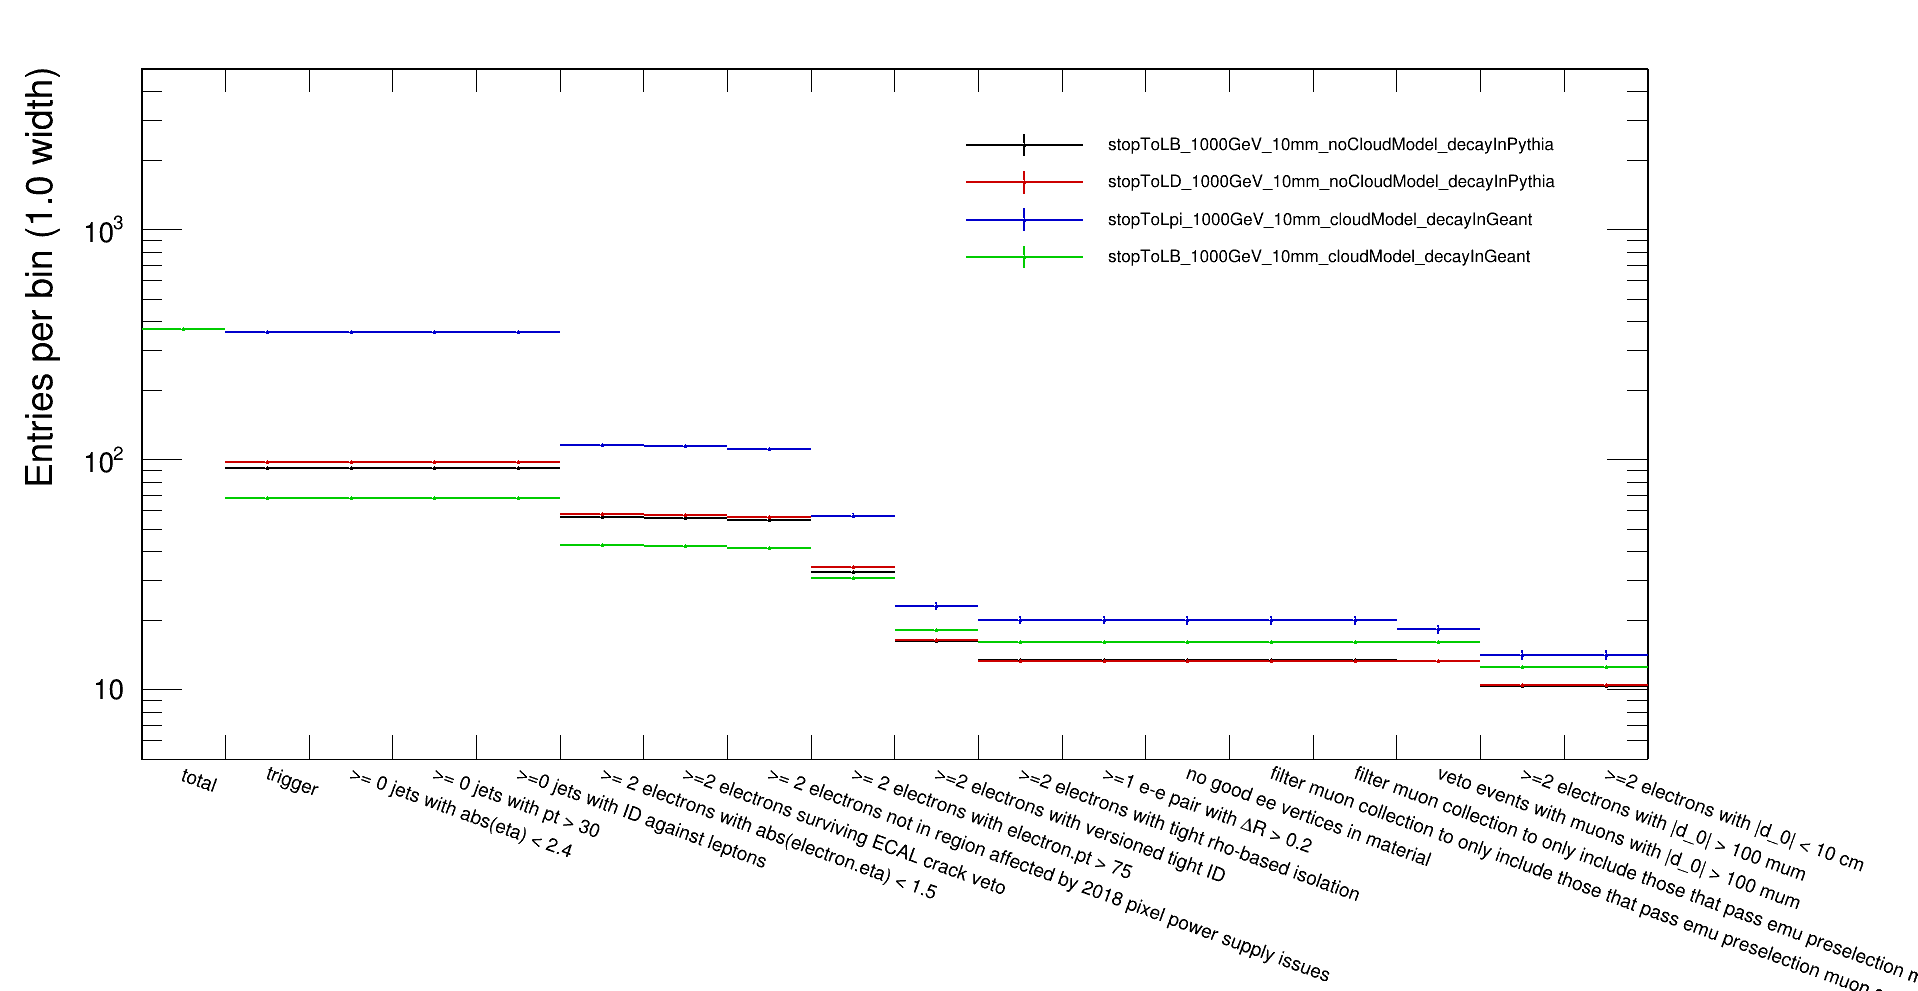
\includegraphics[width=0.9\textwidth]{figures/r_hadrons/ee_cutFlows_lb_ld_lpi_l_1000GeV_10mm.pdf}
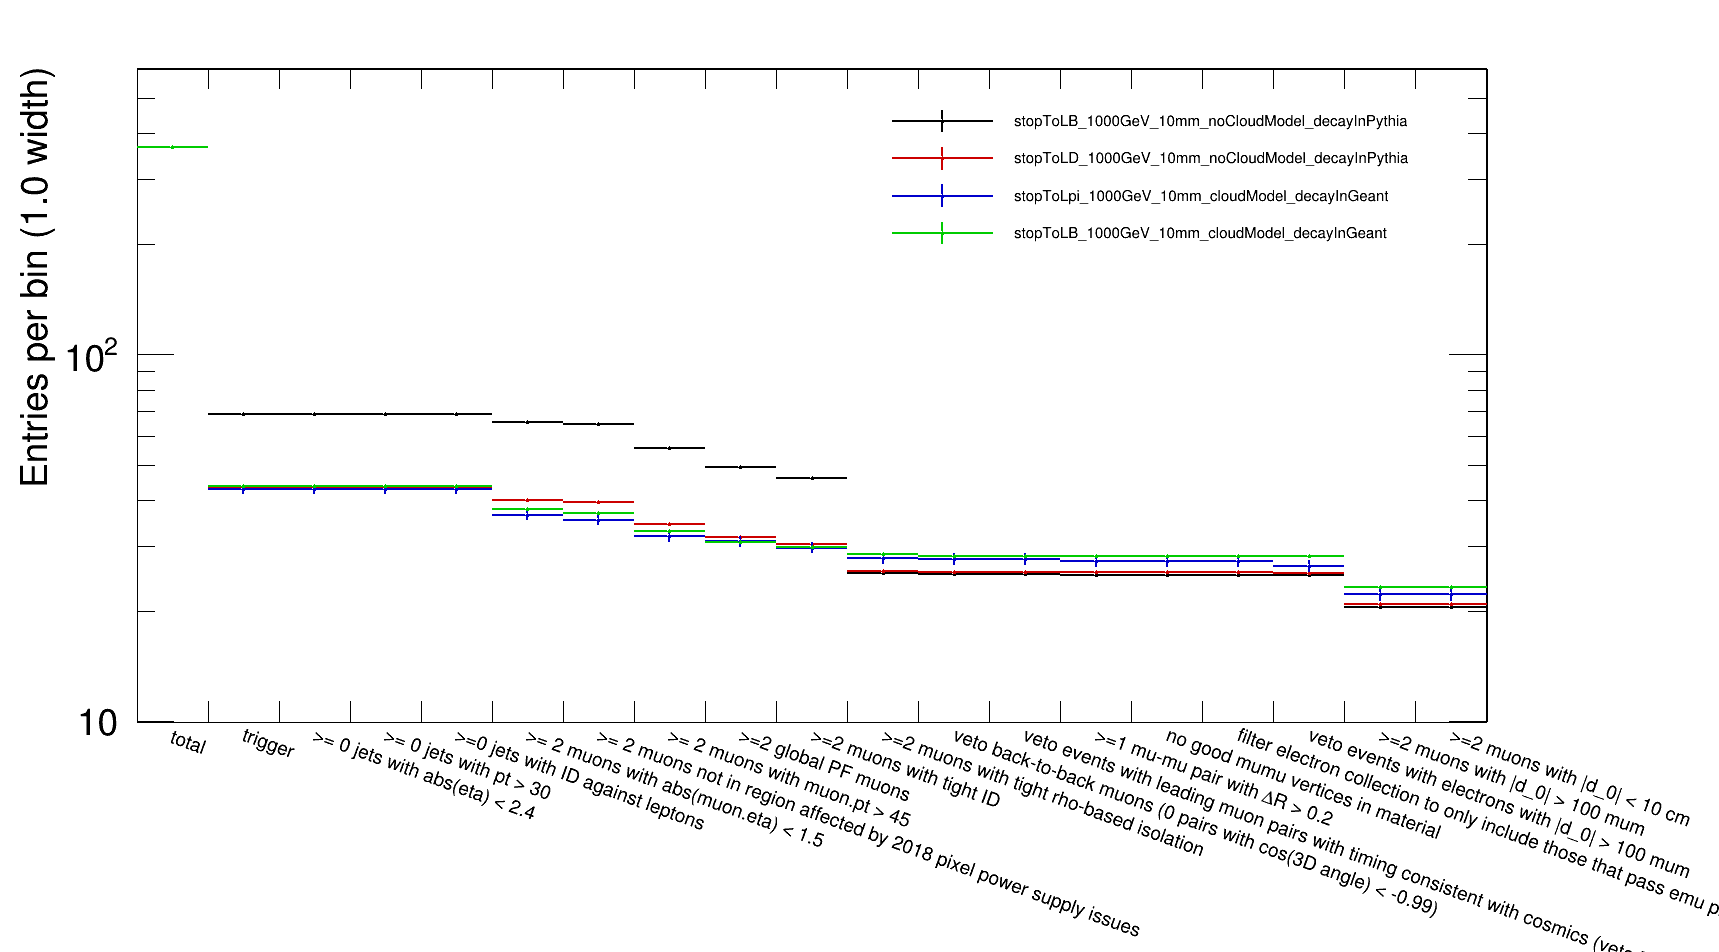
\includegraphics[width=0.9\textwidth]{figures/r_hadrons/mumu_cutFlows_lb_ld_lpi_l_1000GeV_10mm.pdf}
\caption{
Inclusive signal region cutflows for four signal samples  in the $\Pe\Pe$ (top) and $\Pgm\Pgm$ (bottom) channels. The top squark mass and proper decay length are 1000\GeV and 1\cm. In the sample corresponding to the black (red) curves, R-hadron material interactions are not modeled, but the top squark decay is performed in \PYTHIA and the resulting b (d) quark produces a jet. In the samples corresponding to the blue and green curves, the R-hadron material interactions and decay are modeled with \GEANTfour. In the sample corresponding to the blue curves, the R-hadron decays to a lepton and a neutral pion, and in the sample corresponding to the green curves, the R-hadron decays to a lepton and a non-physical final-state quark.
}
\label{r_hadron_cutflows}
\end{figure}

The stated causes of the effects described above are supported by the kinematic distributions of electrons, muons, and jets in each of these samples before and after the inclusive signal region selections are applied. For example, Fig.~\ref{r_hadrons_no_selection} shows that before any selection is applied, events in which the R-hadron decays to a lepton and a neutral pion contain a clear relative excess of high-\pt, isolated electrons; $\PSQt {\to} \cPqb \Pl$ events contain a clear relative excess of high-\pt, non-isolated muons; and events in which the R-hadron decays to a lepton and a non-physical final-state b quark (and to a lesser degree, events in which the R-hadron decays to a lepton and a neutral pion) show a distinct lack of central, high-\pt jets.


\begin{figure}
\centering
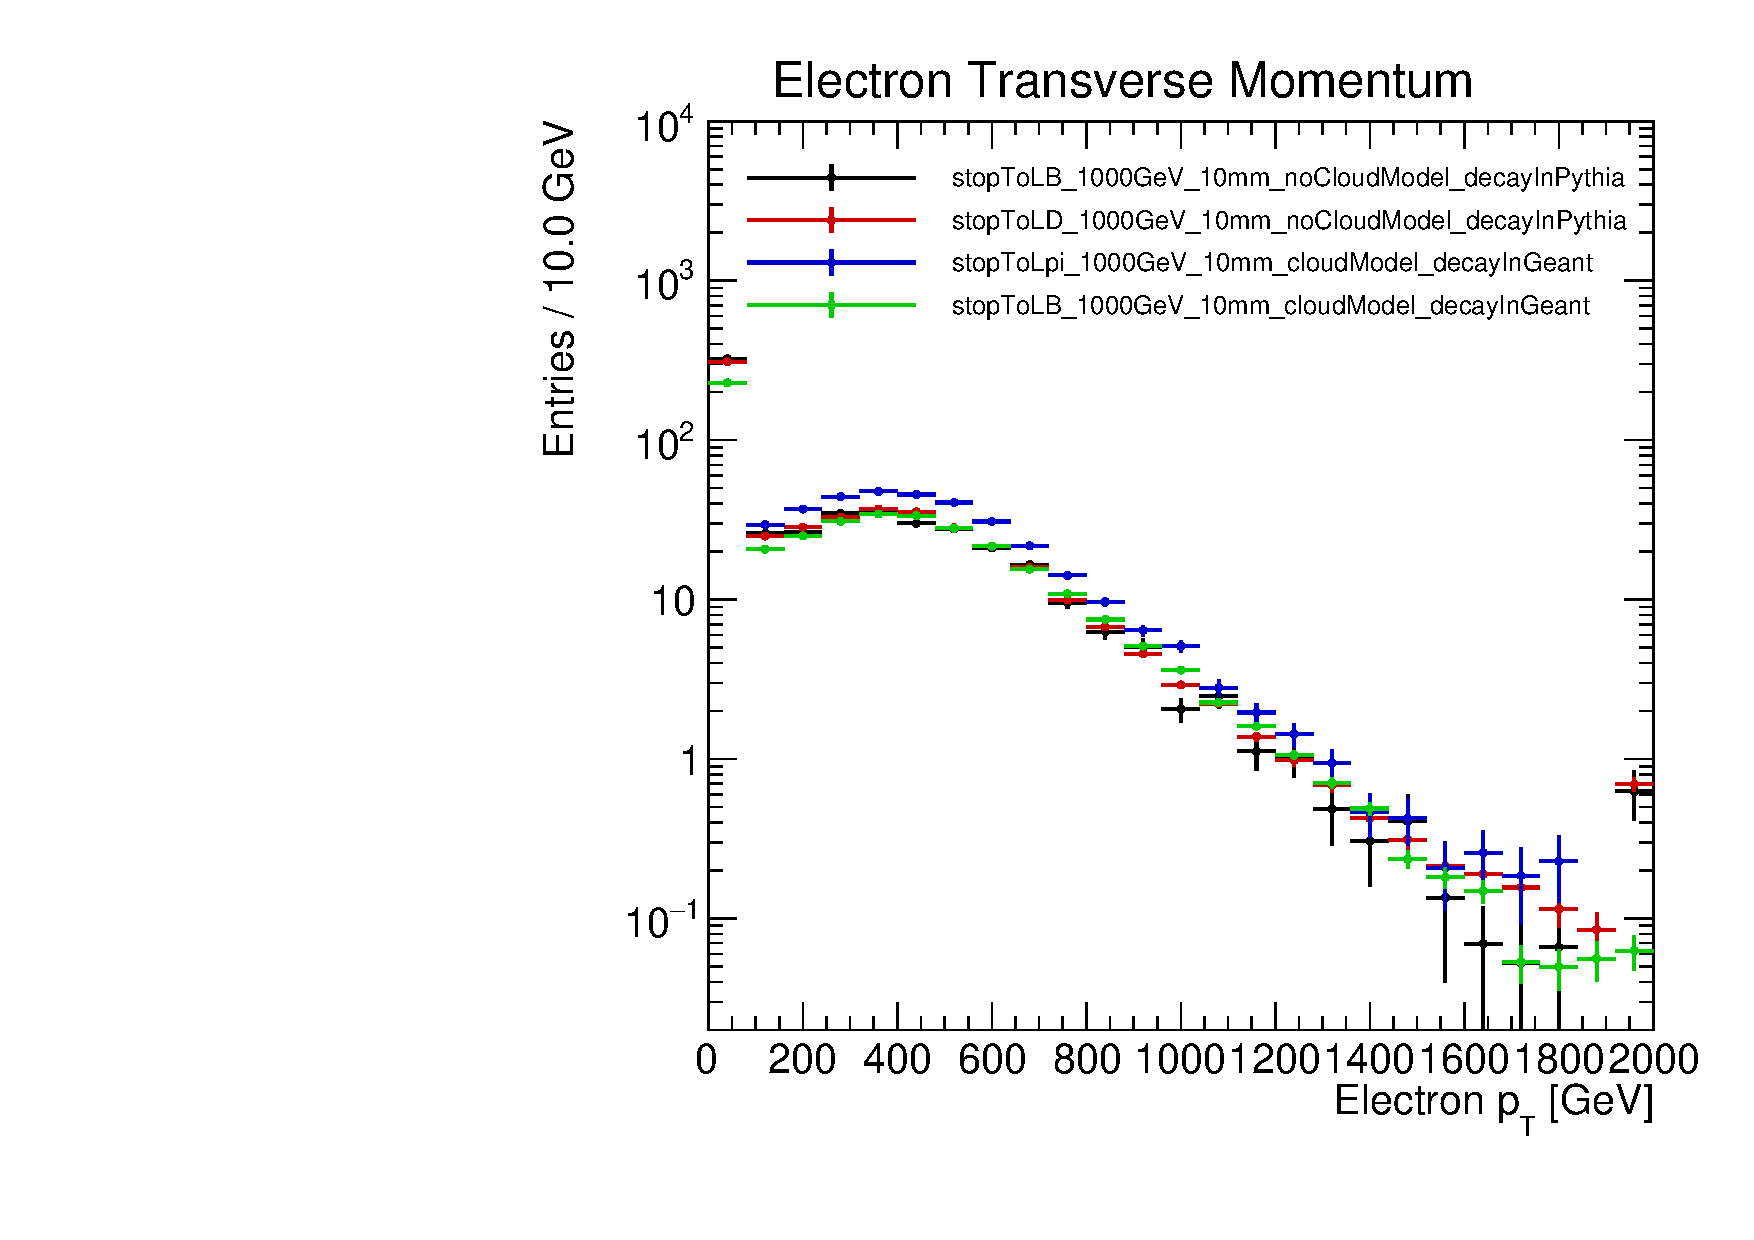
\includegraphics[width=0.35\textwidth]{figures/r_hadrons/e_pt_1000GeV_10mm.pdf}
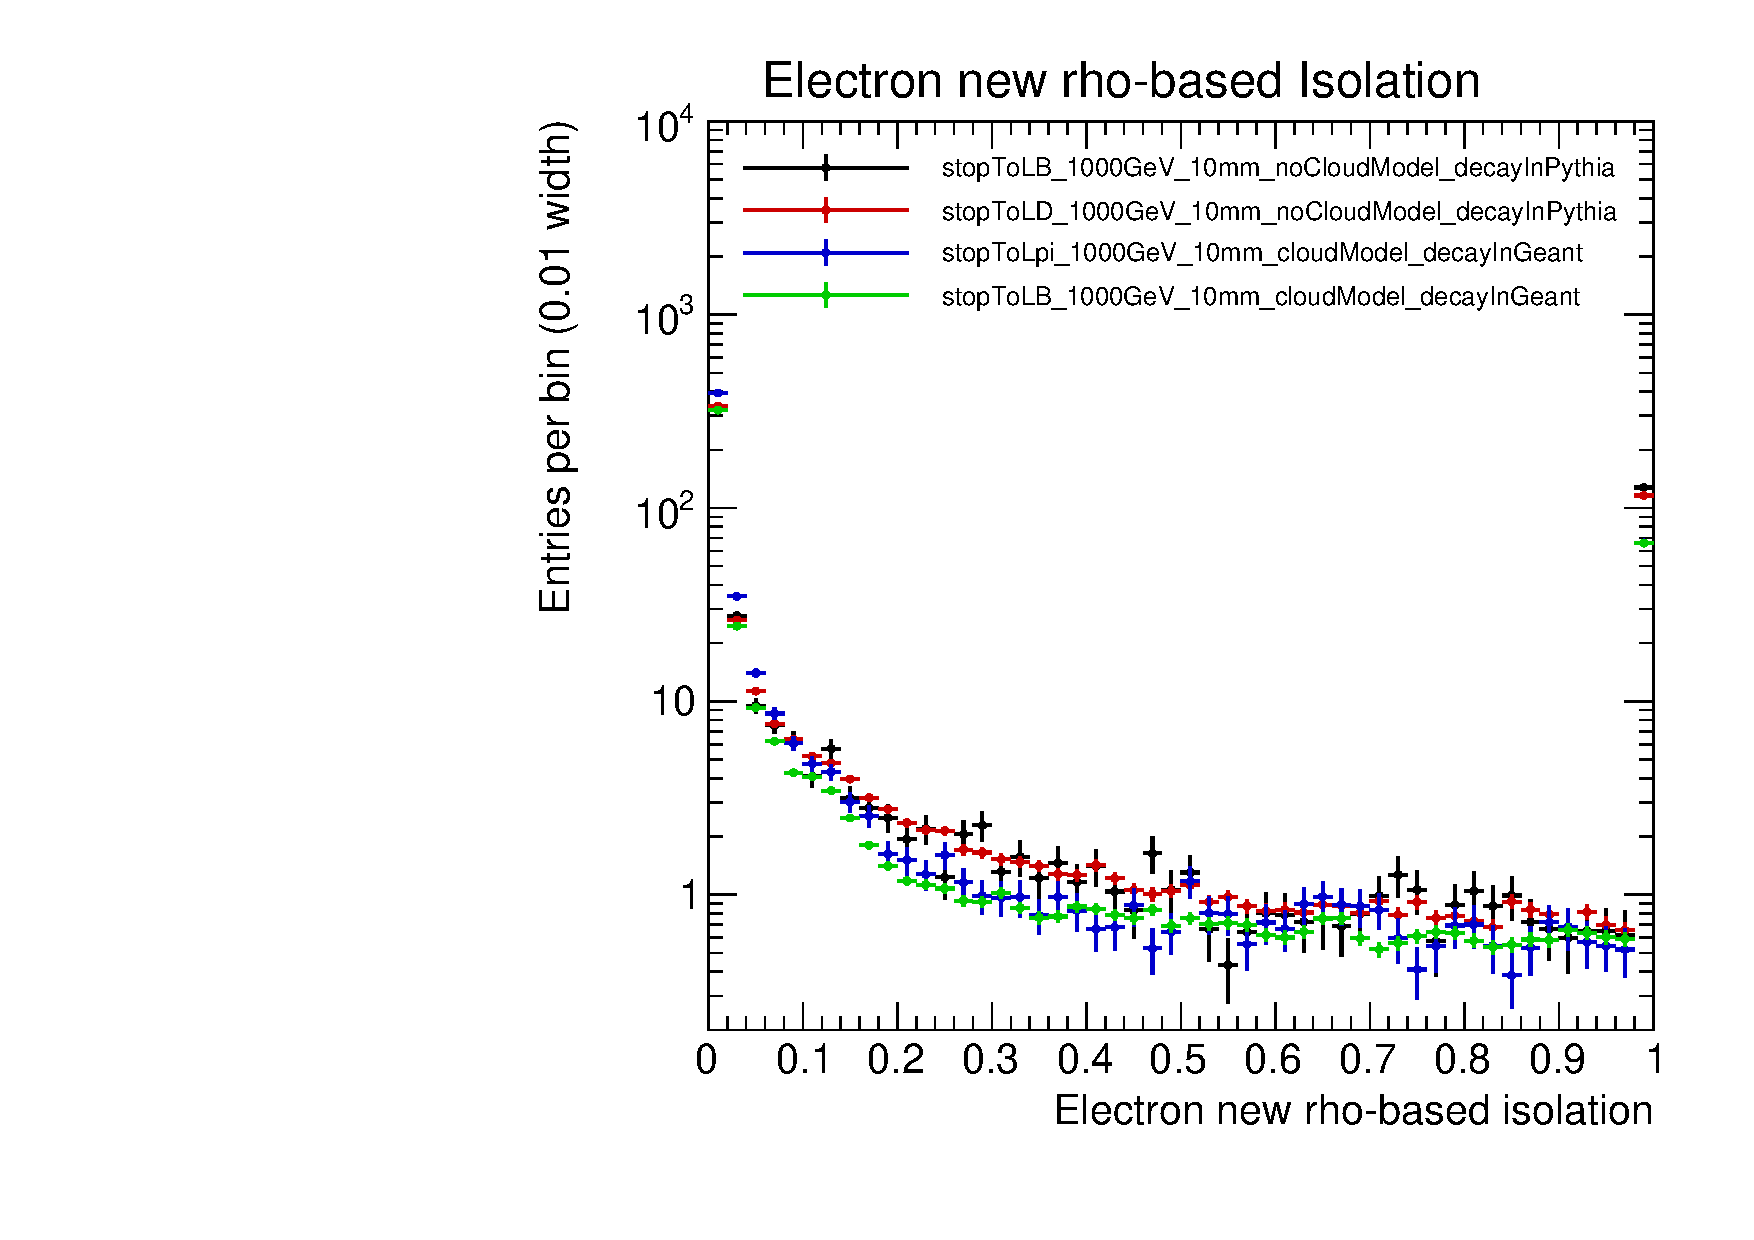
\includegraphics[width=0.35\textwidth]{figures/r_hadrons/e_iso_1000GeV_10mm.pdf}
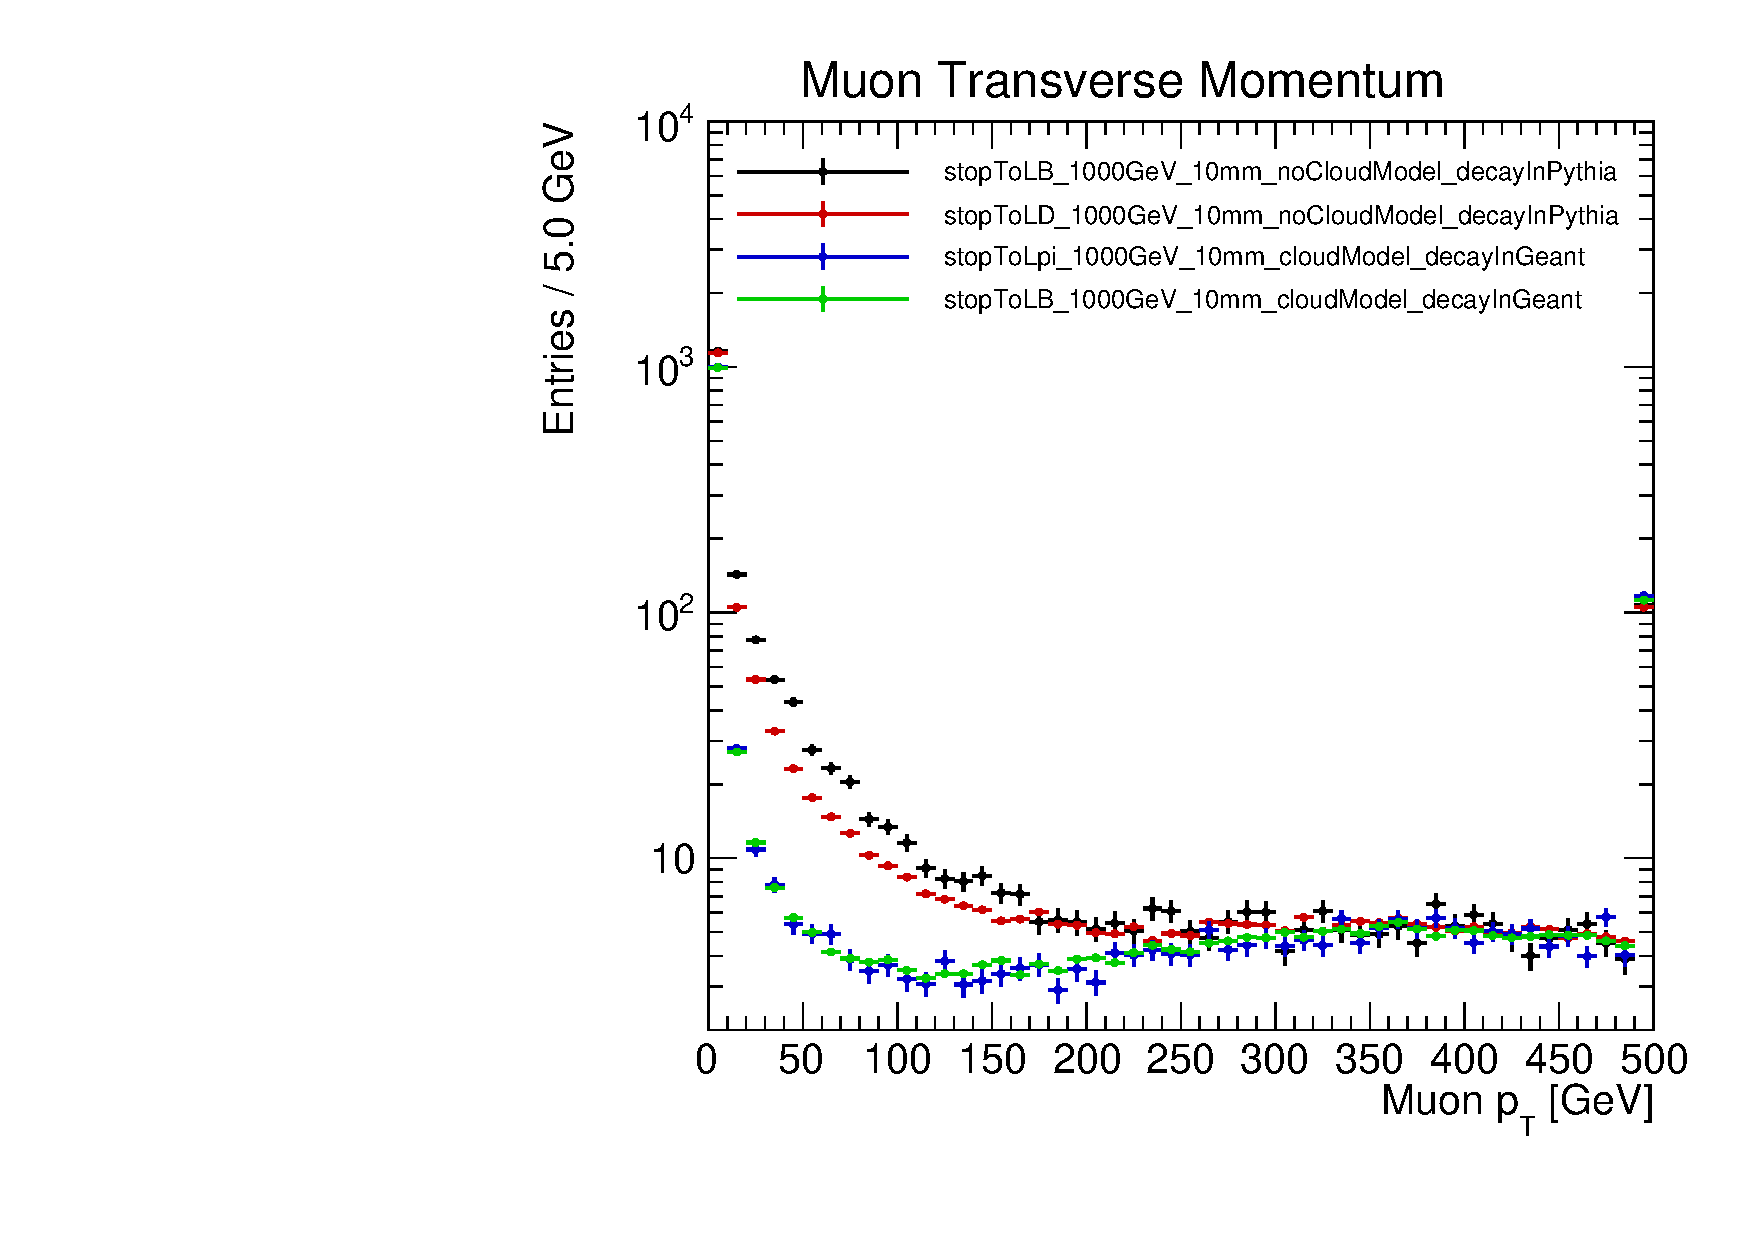
\includegraphics[width=0.35\textwidth]{figures/r_hadrons/mu_pt500_1000GeV_10mm.pdf}
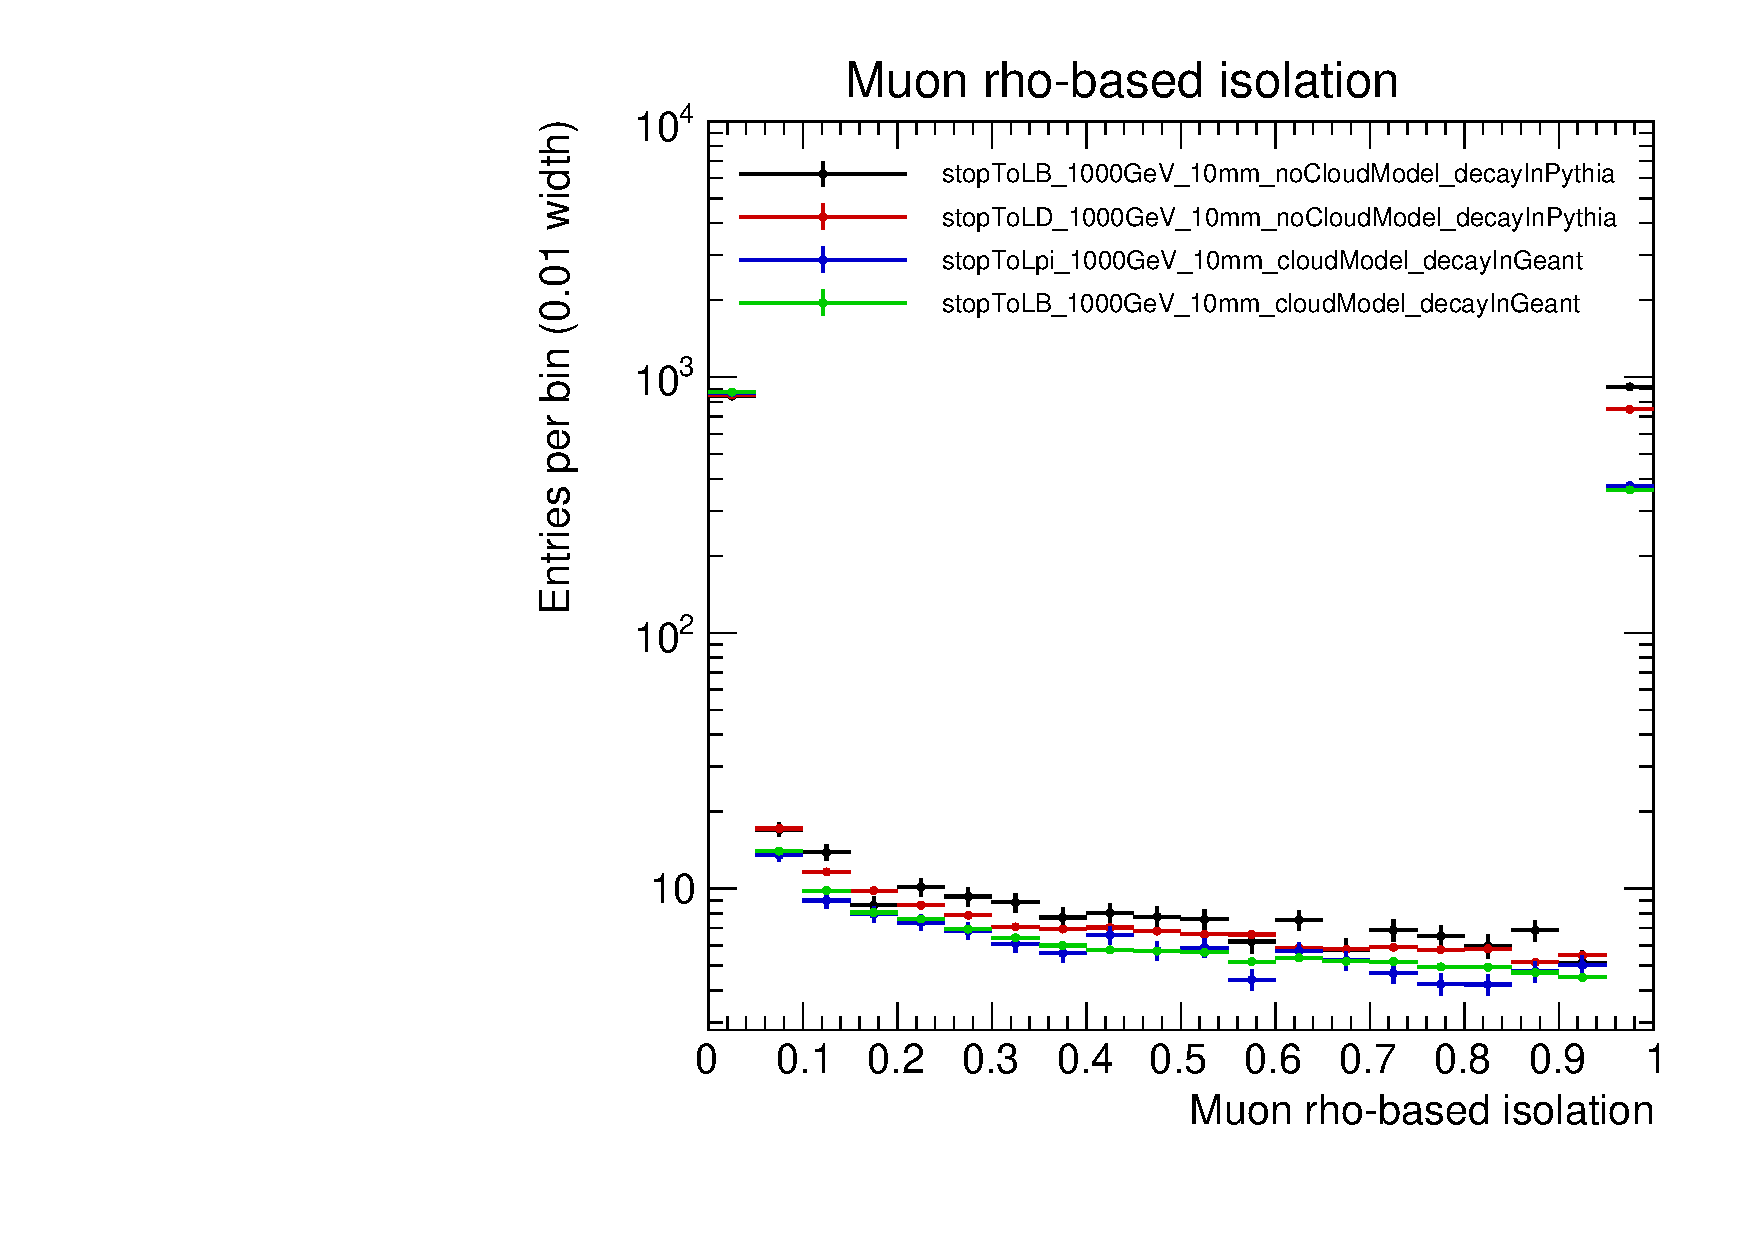
\includegraphics[width=0.35\textwidth]{figures/r_hadrons/mu_iso_1000GeV_10mm.pdf}
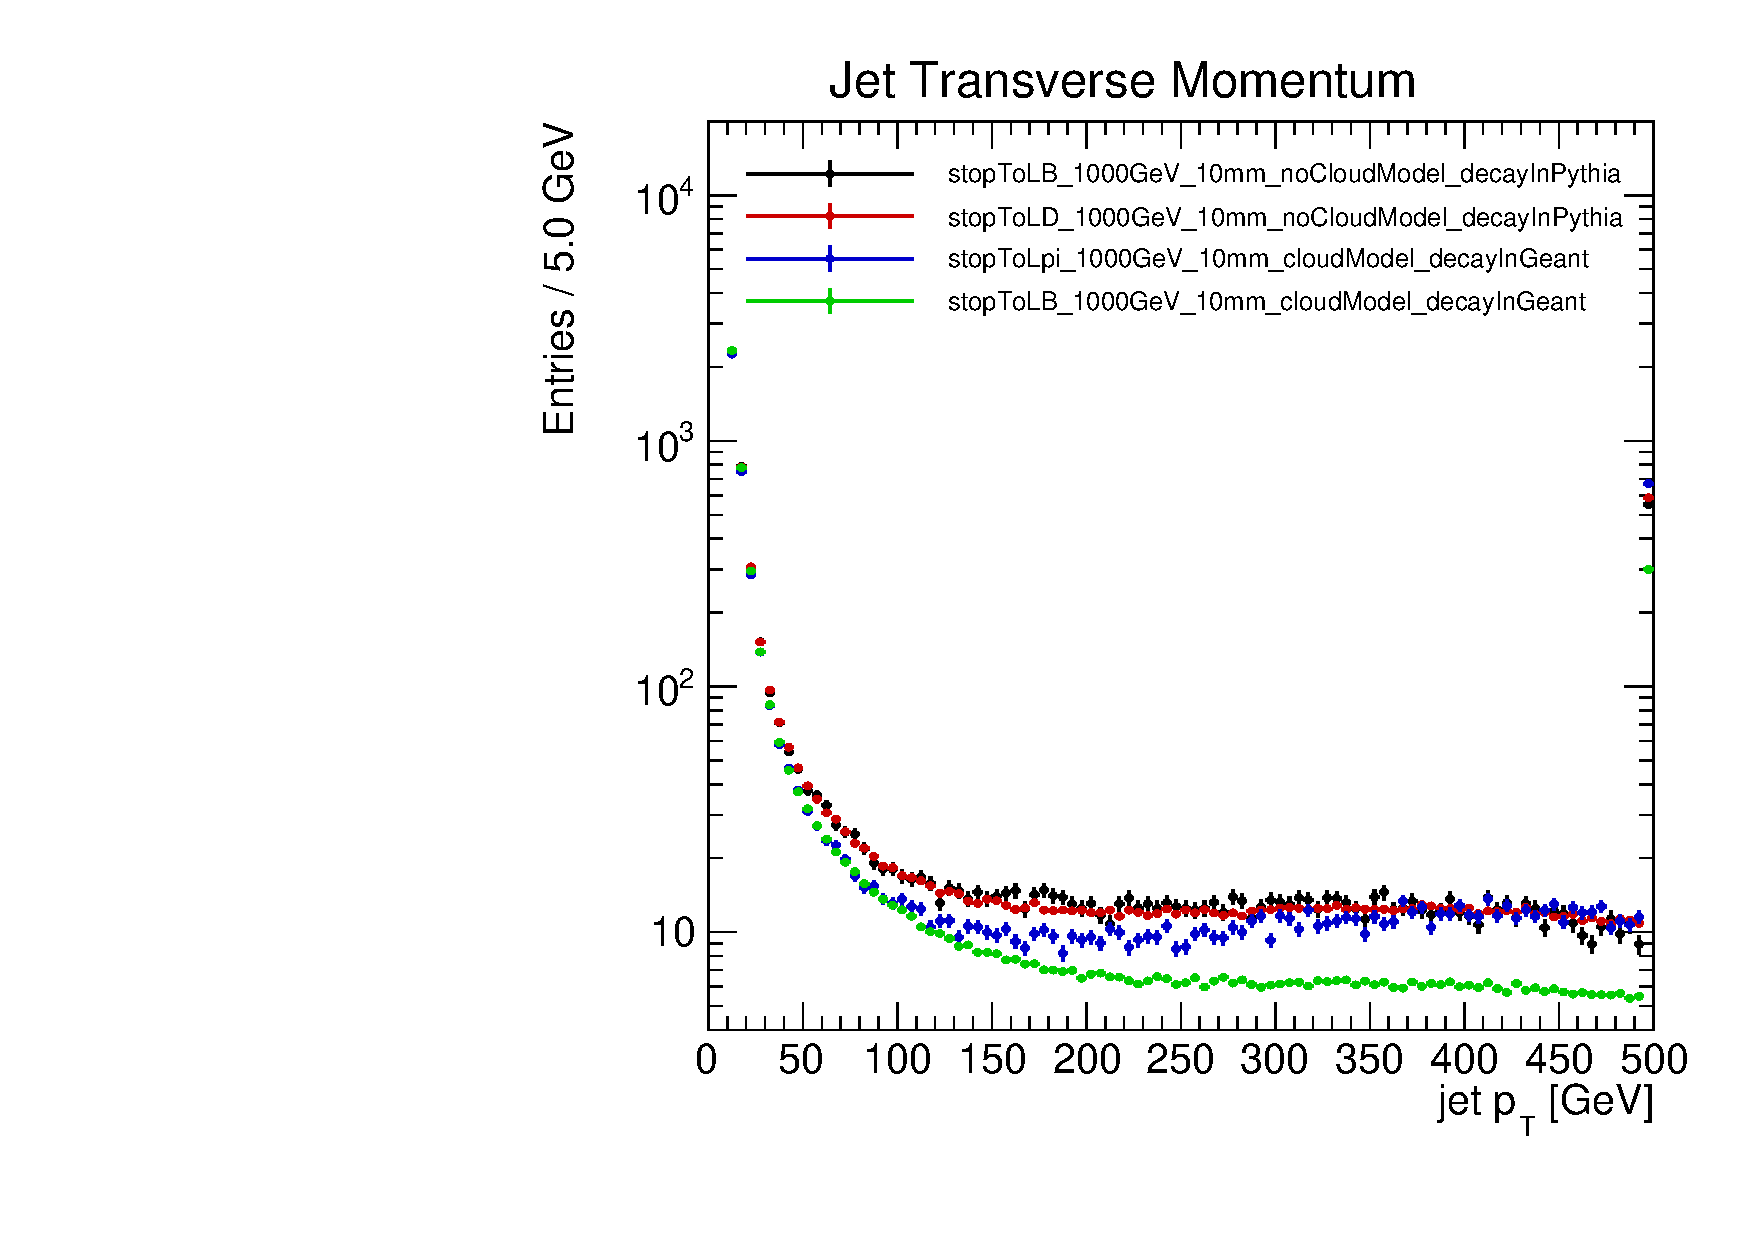
\includegraphics[width=0.35\textwidth]{figures/r_hadrons/jet_pt_1000GeV_10mm.pdf}
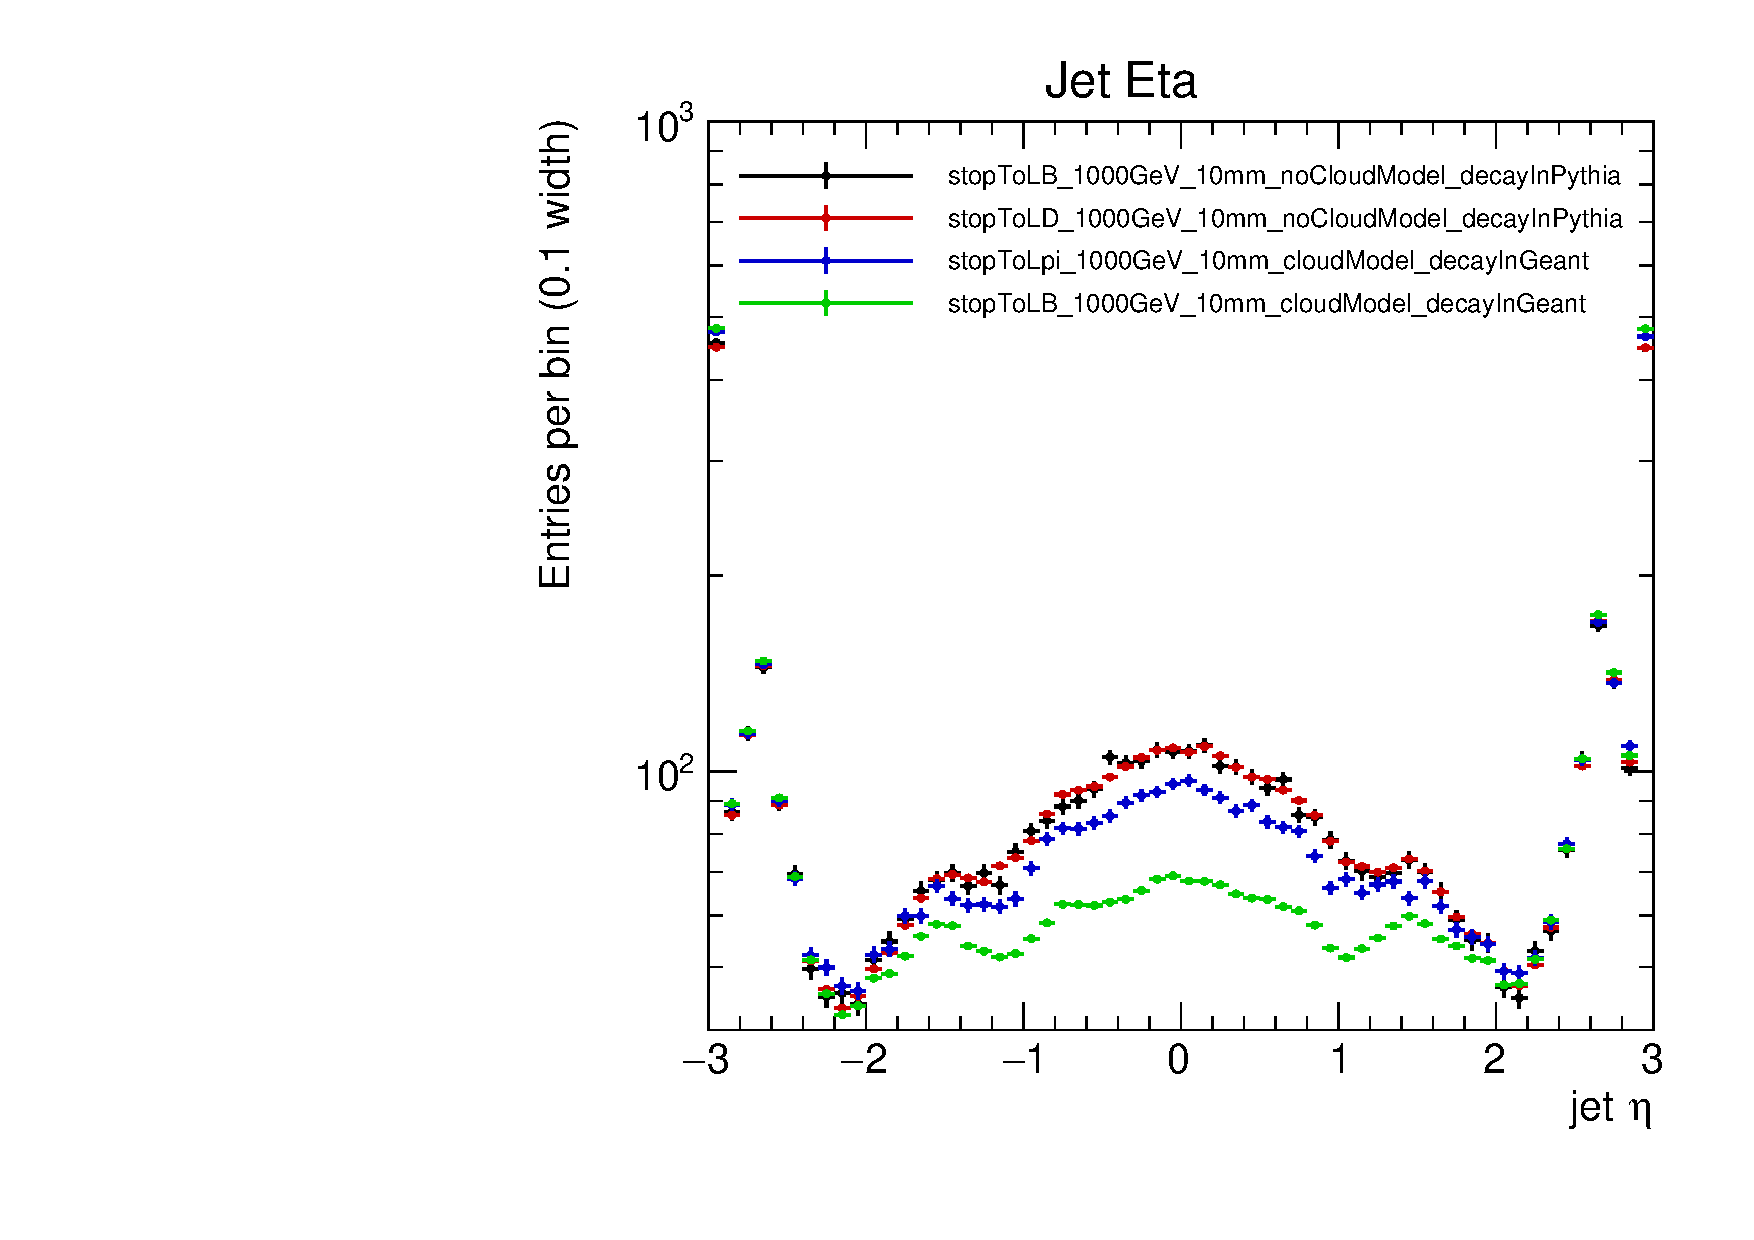
\includegraphics[width=0.35\textwidth]{figures/r_hadrons/jet_eta_1000GeV_10mm.pdf}
\caption{
Kinematic distributions of electrons (top), muons (middle), and jets (bottom) before any selection is applied for four signal samples in which the top squark mass and proper decay length are 1000\GeV and 1\cm. In the sample corresponding to the black (red) curves, R-hadron material interactions are not modeled, but the top squark decay is performed in \PYTHIA and the resulting b (d) quark produces a jet. In the samples corresponding to the blue and green curves, the R-hadron material interactions and decay are modeled with \GEANTfour. In the sample corresponding to the blue curves, the R-hadron decays to a lepton and a neutral pion, and in the sample corresponding to the green curves, the R-hadron decays to a lepton and a non-physical final-state quark. In each plot, the rightmost bin contains overflow entries.
}
\label{r_hadrons_no_selection}
\end{figure}

Figure~\ref{r_hadrons_sr} shows how the effects described above carry through to the events that pass the inclusive signal region selections. As expected, the events in which the R-hadron decays to a lepton and a neutral pion have a relative excess of high-\pt, well-isolated electrons when the full $\Pe\Pe$ signal region selection is applied. The muon isolation cut eliminates the differences between the two samples in which the top squark is decayed in \PYTHIA when the $\Pgm\Pgm$ inclusive signal region selection is applied, but the relative excess of well-isolated muons from the two other samples becomes more pronounced. Finally, the stark differences in jet activity remain apparent.

\begin{figure}
\centering
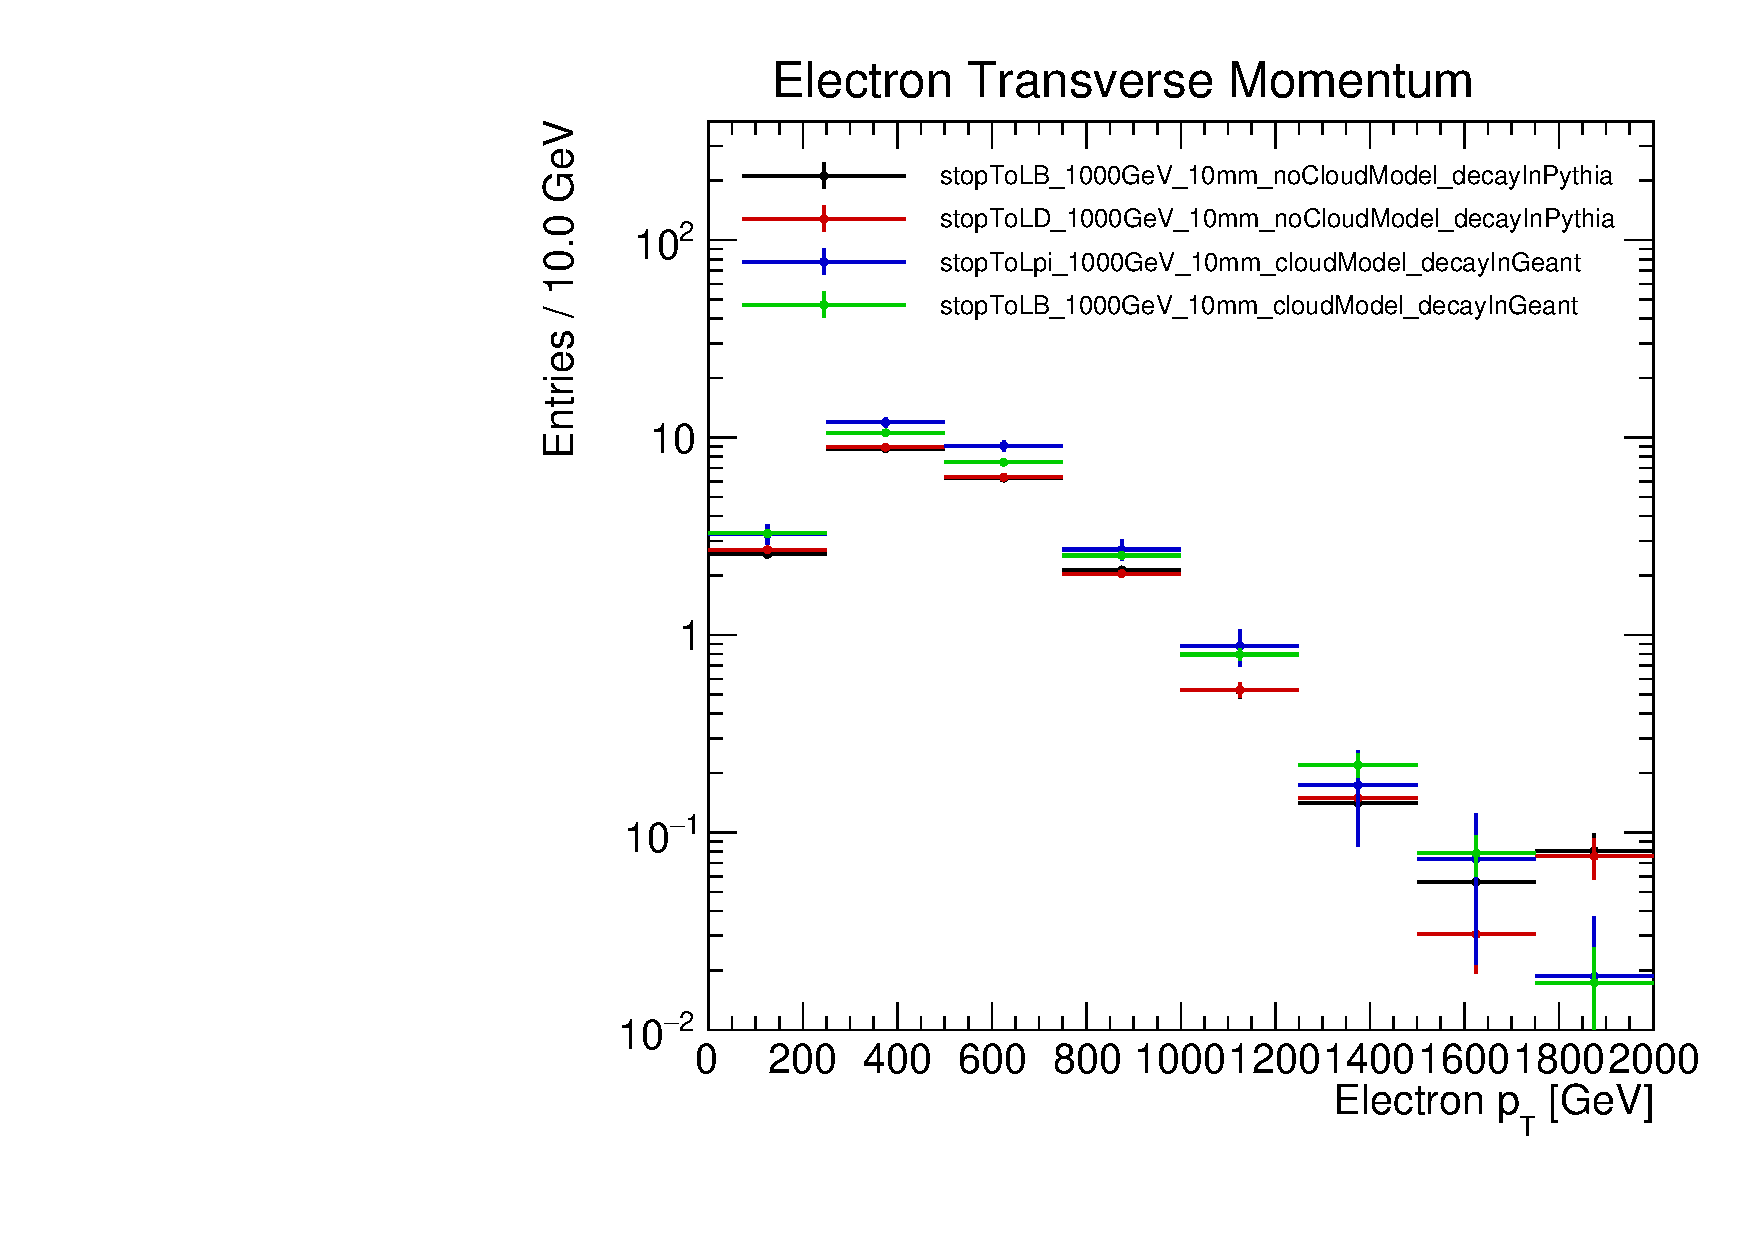
\includegraphics[width=0.34\textwidth]{figures/r_hadrons/eeSR_ePt_1000GeV_10mm.pdf}
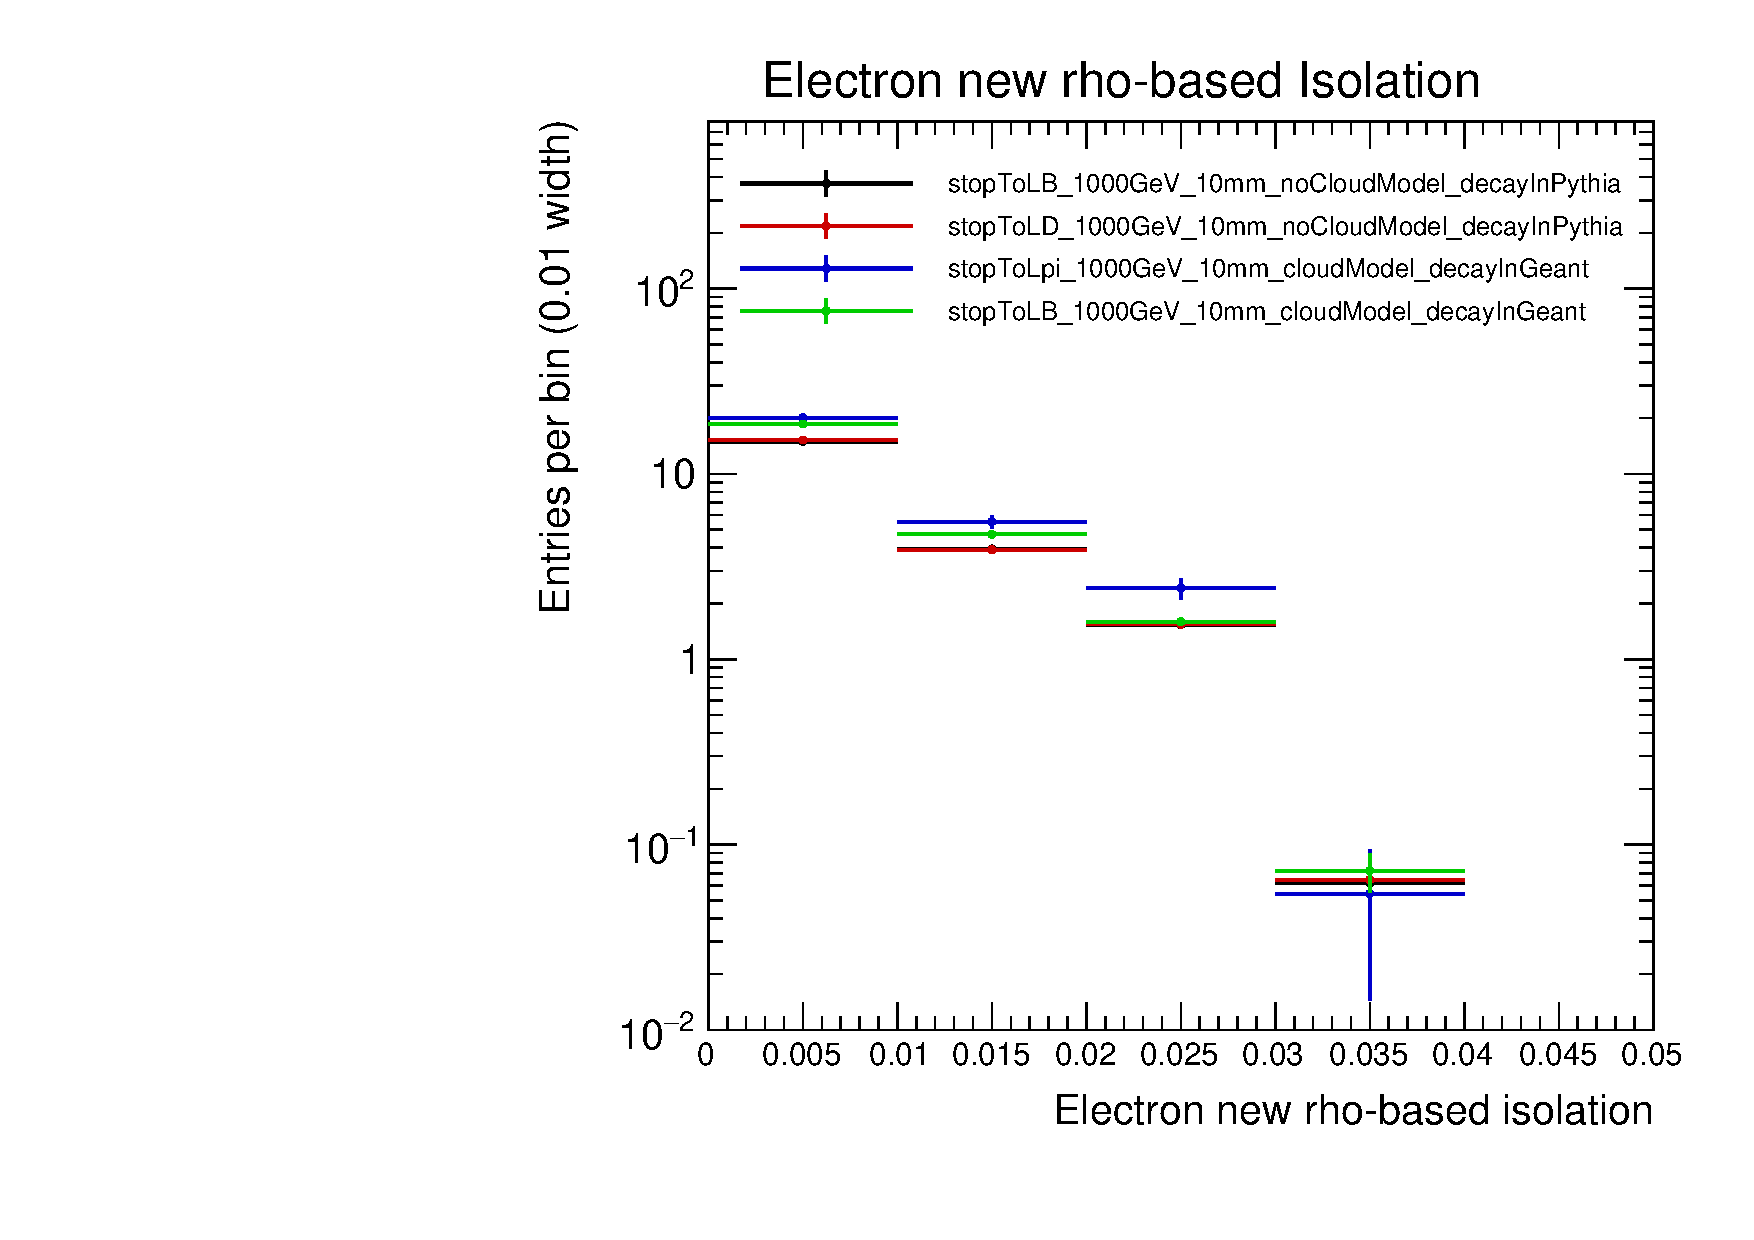
\includegraphics[width=0.34\textwidth]{figures/r_hadrons/eeSR_eIso_1000GeV_10mm.pdf}
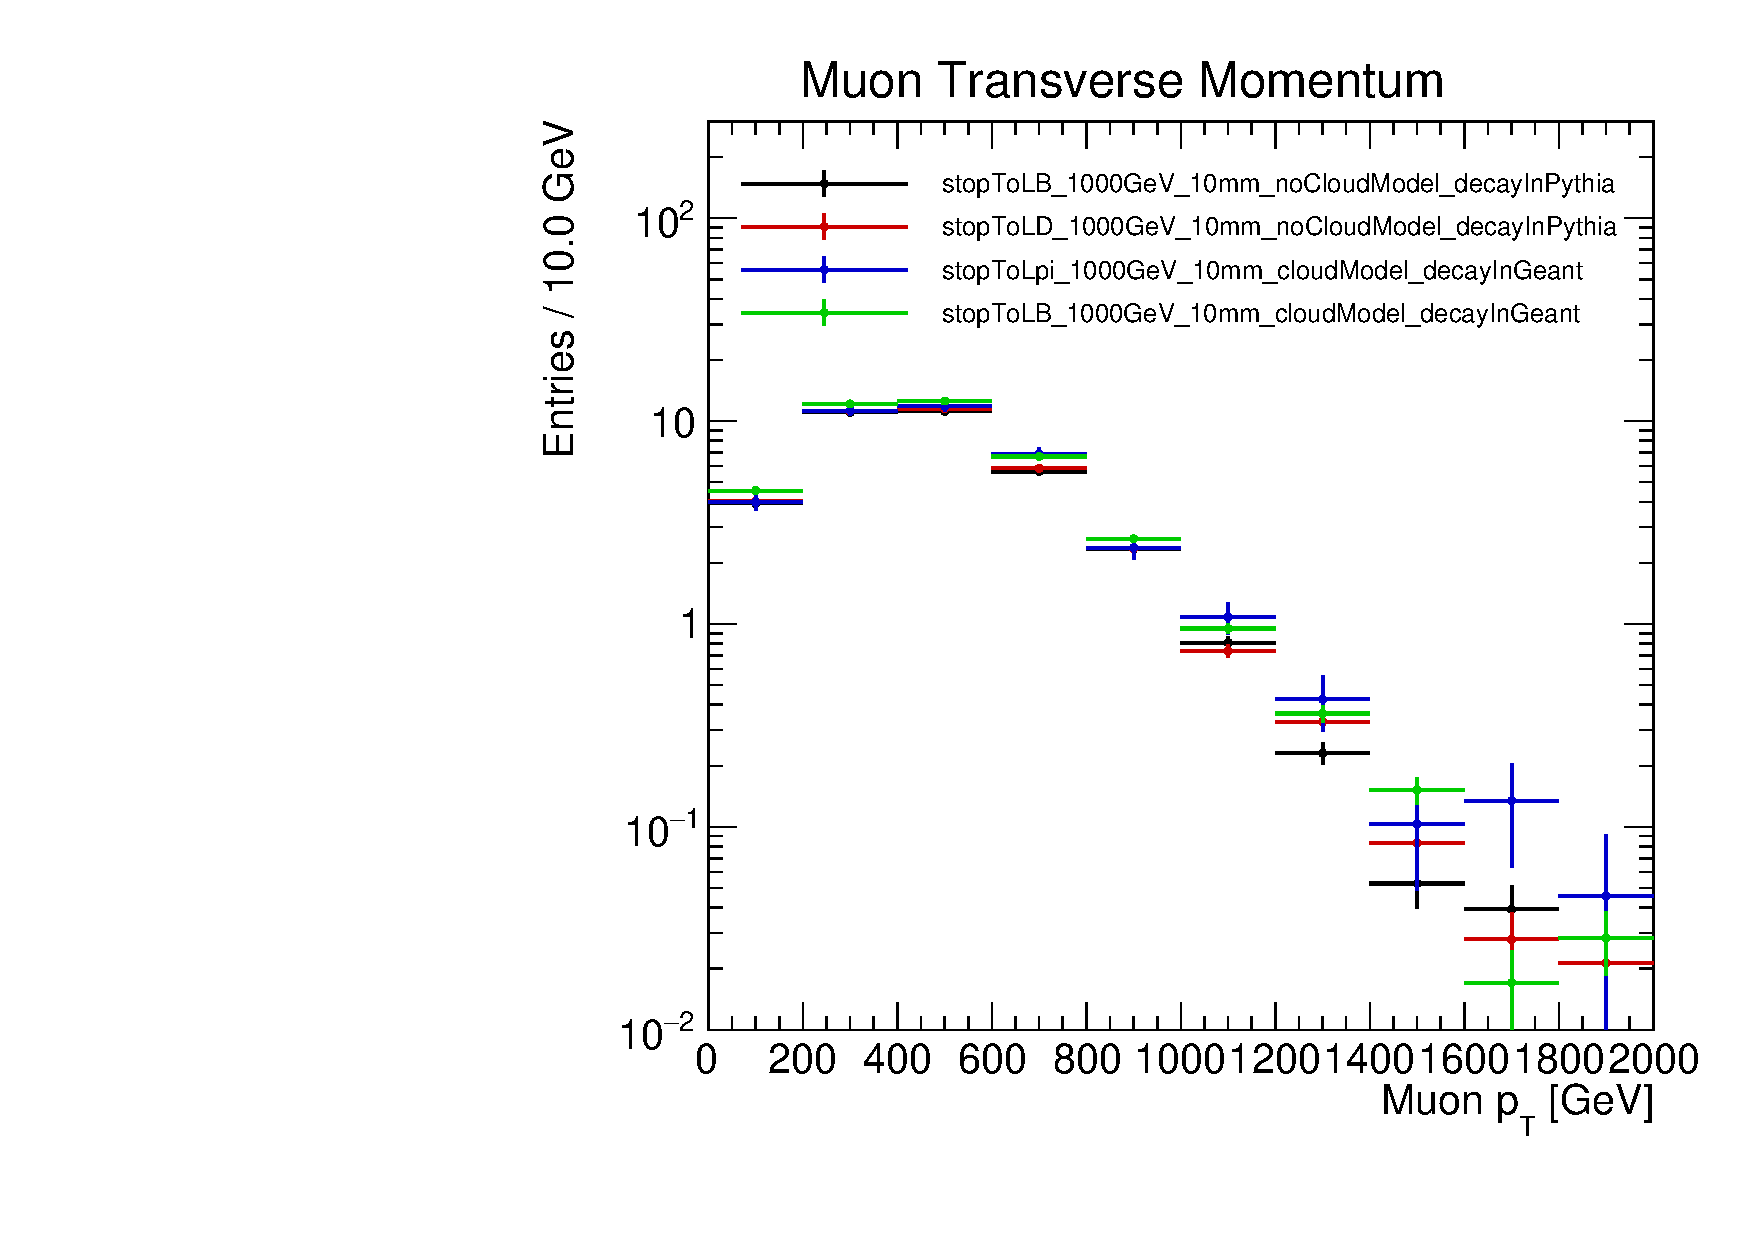
\includegraphics[width=0.34\textwidth]{figures/r_hadrons/mumuSR_muPt_1000GeV_10mm.pdf}
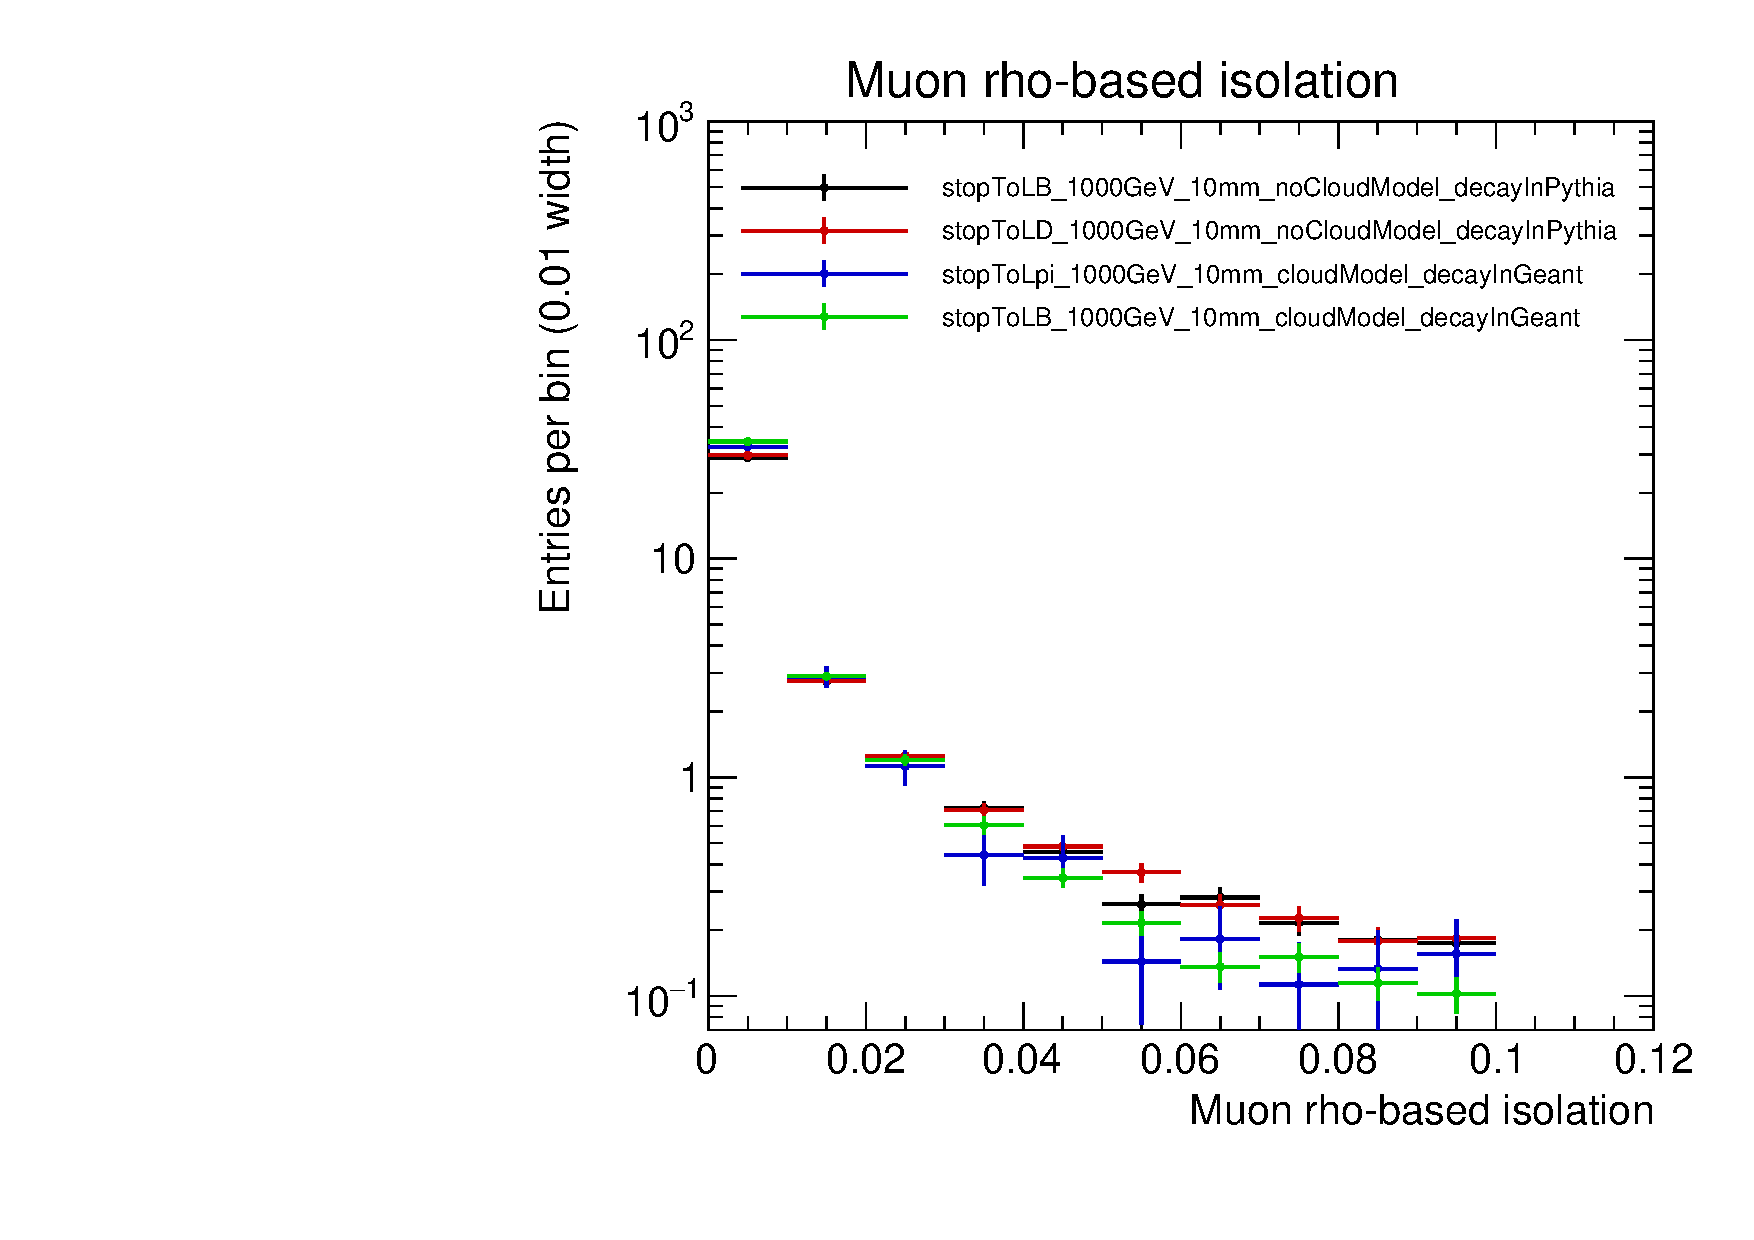
\includegraphics[width=0.34\textwidth]{figures/r_hadrons/mumuSR_muIso_1000GeV_10mm.pdf}
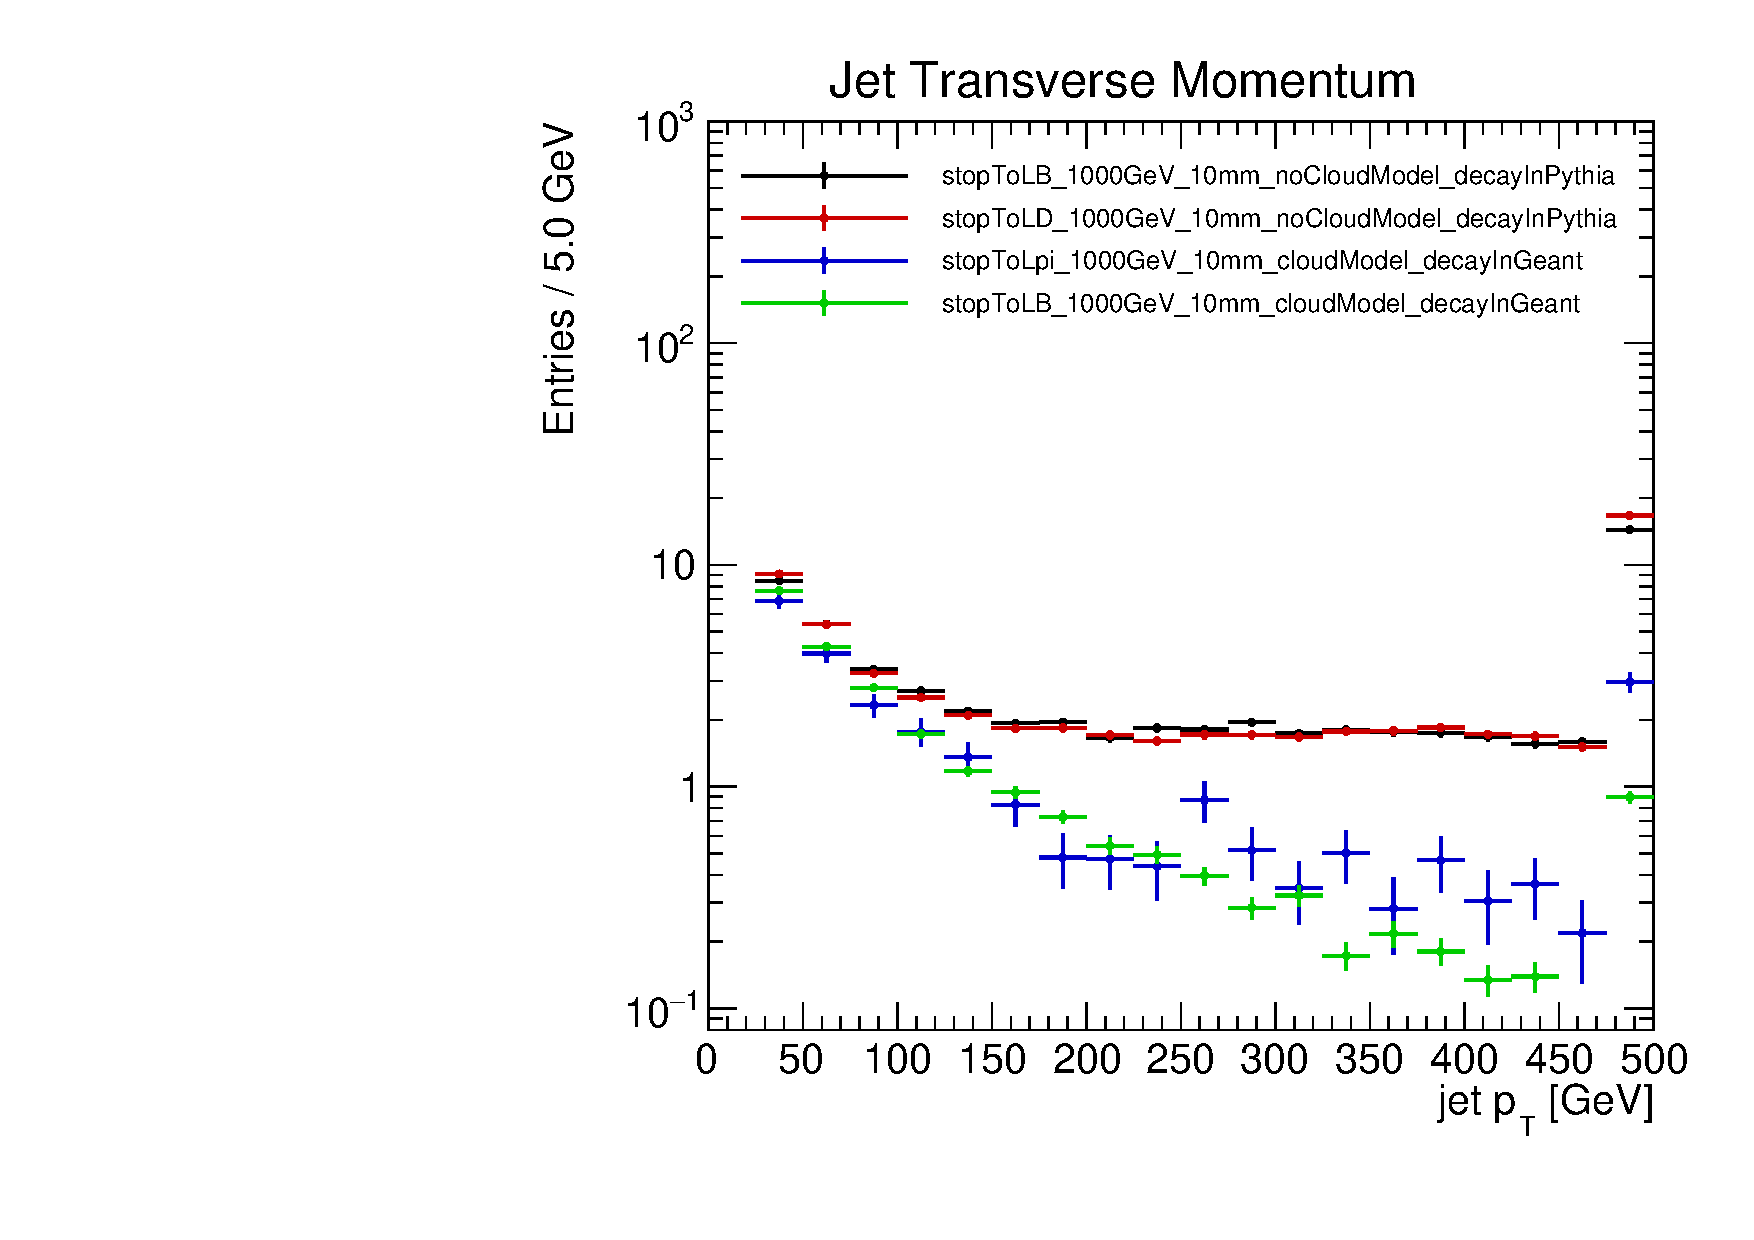
\includegraphics[width=0.34\textwidth]{figures/r_hadrons/mumuSR_jetPt_1000GeV_10mm.pdf}
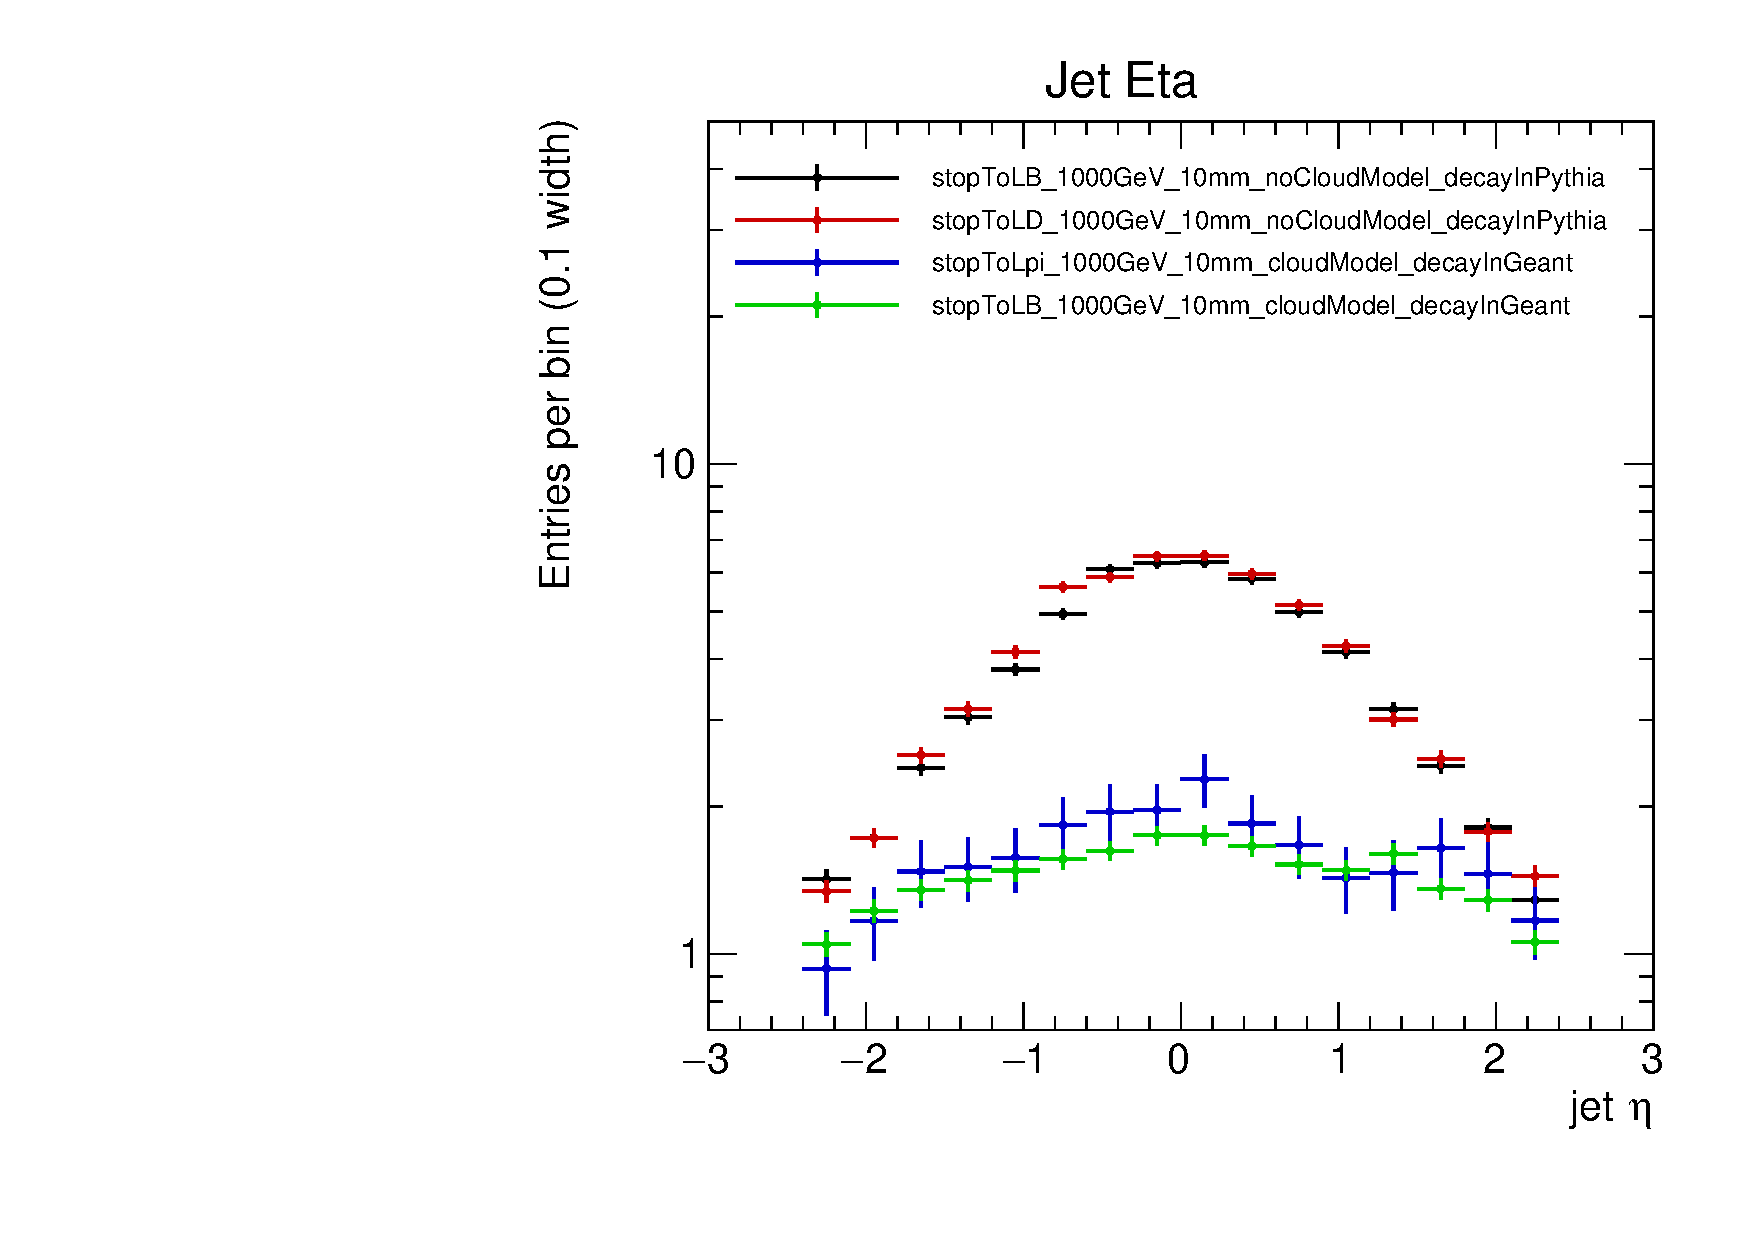
\includegraphics[width=0.34\textwidth]{figures/r_hadrons/mumuSR_jetEta_1000GeV_10mm.pdf}
\caption{
Kinematic distributions of electrons in the $\Pe\Pe$ signal region (top), muons in the $\Pgm\Pgm$ signal region (middle), and jets in the $\Pgm\Pgm$ signal region (bottom) for four signal samples in which the top squark mass and proper decay length are 1000\GeV and 1\cm. In the sample corresponding to the black (red) curves, R-hadron material interactions are not modeled, but the top squark decay is performed in \PYTHIA and the resulting b (d) quark produces a jet. In the samples corresponding to the blue and green curves, the R-hadron material interactions and decay are modeled with \GEANTfour. In the sample corresponding to the blue curves, the R-hadron decays to a lepton and a neutral pion, and in the sample corresponding to the green curves, the R-hadron decays to a lepton and a non-physical final-state quark.  In each plot, the rightmost bin contains overflow entries.
}
\label{r_hadrons_sr}
\end{figure}

In the end, modeling the R-hadron interactions and decay with \GEANTfour has an approximately 20\% effect on the signal efficiency that does not vary meaningfully with analysis channel, top squark mass, or top squark lifetime. We find that all observable differences are due to known, non-physical effects of the modeling of the R-hadron decay and therefore conclude that our nominal signal samples provide the best estimate of the signal efficiency and any real effects from R-hadron interactions must be comparatively small and therefore insignificant to the analysis as a whole.

\pagebreak